\documentclass{article}
\usepackage{amsmath}
\usepackage{amssymb}
\usepackage{graphicx}
\usepackage{hyperref}
\usepackage[version=4]{mhchem}

\title{Problem 3}
\date{}

\begin{document}
\maketitle

\section*{Problem}
Medians \(B D\) and \(C E\) of a triangle \(A B C\) are perpendicular, \(C E=24\) and the area of triangle \(A B C\) is 288 . Find the length of \(B D\).\\
\centering
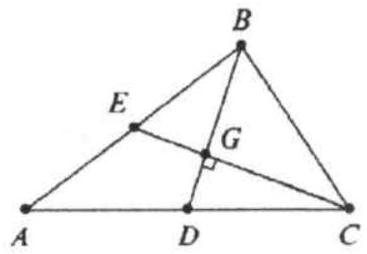
\includegraphics[width=\textwidth]{images/problem_image_1.jpg}

\section*{Solution}
18.\\
\(D G=\frac{1}{3} B D\), and \(C G=\frac{2}{3} C E=\frac{2}{3} \times 24=16\)\\
\(S_{\triangle C D G G}=\frac{1}{2} D G \times C G=\frac{1}{2} \times \frac{1}{3} B D \times 16=\frac{8}{3} B D\)\\
We know that \(S_{\triangle C D G}=\frac{1}{6} S_{\triangle A B C}\)\\
\centering
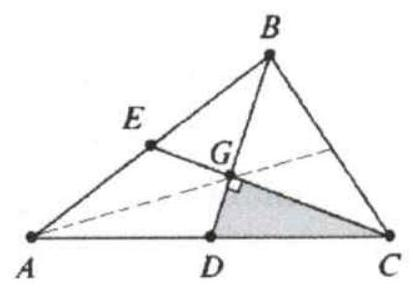
\includegraphics[width=\textwidth]{images/reasoning_image_1.jpg}\\
\(\Rightarrow \quad S_{\triangle C D G}=\frac{8}{3} B D=\frac{1}{6} \times 288 \Rightarrow B D=18\).

\end{document}
